%!TEX root = generalexam.tex

% BEGIN CHAPTER

\begin{blockquote}
    \begin{center}
        Big whirls have little whirls, that feed on their velocity; \\
        Little whirls have lesser whirls, and so on to viscosity. \\
        --- L. F. Richardson (1922) \nocite{richardson1922weather}
    \end{center}
\end{blockquote}

\vspace{2.5em}




%%%%%%%%%%%%%%%%%%%%%%%%%%%%%%%%%%
\section{Intrinsic Predictability}
%%%%%%%%%%%%%%%%%%%%%%%%%%%%%%%%%%

Ever since the days of Lorenz, it has been known that deterministic forecasts are subject to initially small errors growing in amplitude until they become significant features of numerical forecasts \citep{lorenz1963predictability, lorenz1965predictability}. These errors abound from all aspects of numerical modeling, ranging from numerical to observational to the model itself. Unfortunately the aforementioned sources of forecast error are all intricately linked. Advancement on one front does not necessarily guarantee improvements in resulting forecasts. Personal experience indicates that oftentimes improvements in one area results in degradation in other areas.


\cite{thompson1957predictability} defined predictability as ``the extent to which it is possible to predict [any system] with a theoretically complete knowledge of the physical laws governing it.'' Thus, predictability can be considered an inherent property of any system. The atmospheric system most likely has intrinsic predictability properties that are completely divorced from those of any numerical model, arising from the non-linearities contained within the governing equations.  Meteorologists most likely do not fully grasp the intricacy of the atmosphere's predictability.  When on considers that it is possible to describe and solve for the evolution of (some) simple systems analytically, in turn, inherently understanding the predictability of these simple system, it can be frustrating to know that the predictability of more complex systems, such as the atmosphere, cannot be precisely known \citep{hacker2005predictability}.


However, all is not lost. Lorenz recognized that ``some statistical predictability of certain quantities seems to be present even after errors in the complete circulation pattern are no longer small.'' \citep{lorenz1965predictability}. Lorenz postulated that the largest obstacles in numerical weather prediction are inaccurate models and insufficient observations, and not the intrinsic limit of predictability, which yields hope for improvements of numerical forecasts. In fact, most improvements in numerical weather prediction have arisen from improvements in models, assimilation techniques, and observational networks, the advent of improved data assimilation techniques, and the advent of ensemble forecasting \citep{shukla2005predictability}.




%%%%%%%%%%%%%%%%%%%%%%%%%%%%%%
\section{Sources of Errors}
%%%%%%%%%%%%%%%%%%%%%%%%%%%%%%

The National Oceanic and Atmospheric Administration's (NOAA) National Severe Storms Laboratory (NSSL) produces Weather Research and Forecast-Advanced Research WRF (WRF-ARW) model runs at 4-km grid spacing nightly in support of research-to-operations activities between NSSL and the NOAA/NWS Storm Prediction Center (SPC) \citep{kain2010attributes}. The forecast initialized at 00 UTC on 05 February 2008 produced remarkable guidance for forecasters with respect to the potential for a significant severe weather outbreak later that evening (Weiss and Kain 2009, 2010, personal communication). The storm-attribute field, Hourly Maximum Updraft-Helicity, indicated the possibility of numerous, long-tracked rotating thunderstorms over a large portion of the deep south, and as that evening would demonstrate, the forecast was very good. For reasons not discussed here, NSSL has tried to reproduce this forecast without success. In fact, reruns fail to produce long-track Hourly Updraft-Helicity swaths, which were so valuable to forecasters in the initial run. This failure occurs even when using the exact same computer, initial conditions, and version of the WRF. As far as anyone can tell, the only possible difference lies in updated numerical libraries on which the WRF was built against (Kain 2010-2011, personal communication)


\cite{thomas2002floatingpoint} touch on these issues in thorough discussion of errors related to model numerics. Simple changes in processor topology can account for 10-15\% of the magnitude of the total initial-condition and model error. Furthermore, changes in the math library also contribute to a change in the resulting forecast's error characteristics. The takeaway point of their study was that these errors are intrinsic to how numerical modeling is achieved and must be considered anytime something in the computing infrastructure is changed (e.g., numerical libraries, processor configuration, operating system, etc).


The most significant contribution of numerical error comes from the inability to explicitly solve many of the equations involved in numerical weather prediction. Instead, ``solutions'' are often approximated via one of a variety of numerical techniques (e.g., simple approximations, iterative-methods, transformations, etc; \citealp{thomas2002floatingpoint}). Take, for example, the problem of minimizing the cost function in variational analysis. The cost function is known, but is too large computationally for explicit solving in any realistic time frame\footnote{Here's a simple example to illustrate the difficulties on dealing with large amounts of observations. Global scale models routinely deal with observations on the order of $10^8$. To multiply two matrices of dimension $10^8$ requires $10^{24}$ calculations. The world's faster supercomputer, Japan's K Computer, can achieve $10^{16}$ calculations per second. Thus, it would take 3 years, 62 days, 46 minutes, 40 seconds to do a single matrix multiplication, assuming the $10^{16}$ calculations per second could be sustained throughout the course of the calculation.}. Thus, approximations to the exact equations, such as exploiting the tangent linear hypothesis must be implemented, simply to make the problem tractable.


Additionally errors can creep in solely due to how irrational numbers are stored in memory. Intrinsic in any numerical computation are floating-point errors. Take, for example, the following example constructed on the computer on which this document was written.


\vspace{2em}
\begin{code}
    In [1]: 6./9 * 10. - (1./3 * 60/3.)
    Out[1]: -8.881784197001252e-16

    In [2]: 6./9 * 10. - (1./3 * 60/3.) == 0
    Out[2]: False
\end{code}
\vspace{2em}


\noindent The simple expression given in line 1 should evaluate to 0, however, as the output of line 1 and the test given in line 2 demonstrate, this is not the case.  It is hypothesized that by changing numerical libraries can, and does, affect the resulting calculations\footnote{As a side note, the above example illustrates how important it is to conduct floating point arithmetic correctly in numerical settings. Comparisons of two floating point numbers should always be compared against the machine's, or numerical library's, $\epsilon$.}. As numerous studies have shown, even the smallest of errors can rapidly grow upscale, contaminating a forecast.


Before discussing predictability and error growth issues evolving from choice of horizontal grid spacing, it is important to visit the issue of resolution. Historically, many have used the terms ``resolution'' and ``grid spacing'' interchangeably \citep{grasso2000resolution, pielke1991resolution}. This is incorrect. A model's grid spacing is the distance between two adjacent grid points, $\Delta x$. A model's resolution should be considered as the smallest scale at which numerical waves are ``resolved''\footnote{The definition of resolved is open to interpretation. Is this the smallest distance at which a wave can be represented? Is this the distance at which some percentage of a wave's amplitude can be resolved?}. In the atmosphere, energy is passed both upscale to larger phenomena and downscale to smaller and smaller phenomena. In the context of smaller phenomena, eventually the energy is dissipated through molecular dispersion. However, in a numerical context, turbulent mixing is parameterized. Thus, small scale energy ultimately gets aliased back to larger scale phenomena contaminating the forecast, which starts the process all over again. Eventually this will lead to numerical instabilities and render the forecast worthless \citep{phillips1959instabilities}. To prevent this from happening, numerical models typically employ some sort of artificial damping scheme designed to remove waves of $2\Delta x$ or $3\Delta x$. Thus, oftentimes the finest resolution a model can achieve is  $4\Delta x$ \citep{grasso2000resolution}.


Even though an atmospheric phenomenon occurs on the order of the grid spacing, it might not adequately be resolved. One such example of this is the relatively large size of supercell-like structures in simulations with grid spacing of 4 km versus those at 1 km. Thunderstorms on both scales require a minimum number of grid points to resolve the thunderstorm (and release the convective instability). Assuming that the model first develops a thunderstorm on the smallest possible scale, the thunderstorm simulated in the 4 km grid will have approximately 16 times the areal extend as the thunderstorm resolved on a 1 km grid.


As model grids continue to become finer, several studies have shown that with increasing resolution (decreasing grid spacing) come more realistic forecasts of atmospheric phenomena, especially those on the convective-scale (e.g., \citealp{clark2012overview, clark2010mcv, clark2010verification, clark2009comparison, kain2008camconsiderations, done2004cams}). Typically, as grid spacing nears O(1 km) it is assumed that the model can simulate deep moist convection, based on the argument that non-hydrostatic processes can be represented at this scale \citep{weisman1997resolution}. Unfortunately, decreasing resolution comes at the cost of increasing the error growth rates and enhanced non-linearities \citep{ancell2006structure, park1999nonlinearity, park2000sensitivity, sun2005challenges}. Thus there is an inherent trade-off between the times at which a forecast can be considered ``valid'' and  the resolution at which the ``valid'' forecast can be made. In other words, 10 day forecasts made with a model using grid spacing O(1 km) will suffer from increased error feedback than a forecast made over the same time length utilizing grid spacing O(30 km).


Numerical simulations with grid spacing O(1 km) are capable of resolving the basic structure of mesoscale convective systems, even though small scale details may not be correct \cite{bryan2003resolution}. However, grid spacings O(100 m) are required to realistically simulate convective scale processes (e.g., updraft entrainment, convective overturning, etc), especially intra-cloud turbulence. However, improvements regarding the overall performance and structure are greatest when going from numerical forecasts with grid spacing O(10 km) to O(1 km) than from O(1 km) to O(100 m)\cite{bryan2003resolution, kain2008camconsiderations}. This leads to questions as to how best represent a model's performance. Should WoF evaluate models in terms of improved forecast performance or improved depiction of system dynamics? Regardless of one's answer, for the purposes of WoF, grid spacing must decrease farther if the goal is to explicitly predict all severe-convective hazards.  Results from \cite{xue2008tornado} suggests that horizontal grid spacing of O(50 m) may be an upper bound for simulating even the largest tornadoes!


During the most recent WoF workshop, Louis Wicker commented that in some aspects it was easier to predict isolated supercells than it was to predict a mesoscale convective system\footnote{This was in reference to struggles encountered in predicting the evolution of a rather small mesoscale convective system over the lower Great Lakes.}. This statement flies in the face of conventional wisdom -- that the larger mesoscale convective system is easier to predict because its larger scale is more readily sampled by observations making it is easier to sample the mesoscale circulation associated with the mesoscale convective system. Not to put word's in the speaker's mouth, but it is offered that he was dancing around the subject of what drives mesoscale convective systems. Conventional wisdom is what it is for a reason. However it is proposed that in the context of small, or slow-to-develop mesoscale convective systems, the larger scale mesoscale circulation is also slow to develop. This might imply that in the developing stage, the mesoscale convective system acts more like individual thunderstorms than it does as a coherent system. The results of \cite{bryan2003resolution} suggest the inability to directly simulate the individual thunderstorms on (relatively) coarser grid spacings [O(1 km)] impacts the evolution of the mesoscale convective elements in the model, which in turn effects how the mesoscale circulation evolves, ultimately wreaking havoc on numerical simulations.


Another possible explanation to the problems expressed by Wicker involves the environment in which the simulations are initiated. \cite{stensrud20103dvar} and \cite{dawson2012enkf} demonstrate that the simplifications of assuming a homogeneous environment for storm-scale prediction is inadequate for a WoF system. Subtle changes in the environment appear to play significant roles in the subsequent development and evolution of surface cold-pools, as well as low- and mid--level mesocyclones, which ultimately appear to drive storm evolution. Since mesoscale convective systems are orders of magnitude larger than an isolated supercell, it is less likely that environment the mesoscale convective system evolves in is homogeneous. Thus, how well the initial environment is represented, particularly inhomogeneities, ultimately impacts the predictability of the phenomena at hand. Tying back to the issue of model resolution, \cite{stensrud20103dvar} found improvement in storm evolution and mesocyclone path as a result of decreasing the grid spacing from 3 to 1 km. However, the largest improvement in the forecasts came about because of the inclusion of horizontal environmental variability in the environmental conditions.


Several studies over the course of the last few years continue to demonstrate the dependency convective-scale simulations have on the choices of microphysics scheme (e.g., \citealp{tong2008simultaneous, hong2009sensitivities, yussouf2012radarcomparisons, bryan2012microphysics}). This is not surprising considering the myriad of studies that have observed that changes in microphysics intercept parameters can vary widely over a relatively short distance (e.g., \citealp{joss1969dsderrors, ziegler1983hail}) in nature. The sensitivities to microphysics choices, and intercept parameter choices within, demonstrated during the convective initiation component of the Hazardous Weather Testbed's 2011 Experimental Forecast Program. Model soundings from a subset of ensemble members -- those of identical model configurations except for varying choices for either microphysics planetary boundary layer schemes, or both -- time and time again depicted significant structural changes in the evolution of the forecast profile. More specifically, the diurnal evolution of the temperature traces typically varied less than those of the dew point temperature traces, with minimums in spread occurring the overnight hours and maximums occurring during peak heating. \cite{marshall2003pbl} documented that all of the parameterization schemes that help to control the evolution of the planetary boundary layer have deficiencies, leading to errors in resulting forecasts.


Reaching back to the discussion on data assimilation, there is question as to the duration of which the tangent linear model, or the \emph{tangent linear hypothesis}, is valid. \cite{hohenegger2007predictability} demonstrated that the tangent linear approximation fails after period O(1.5 h) in cloud-resolving numerical forecasts. In the context of non-linearity, a 10-day synoptic-scale forecast equates to a cloud-resolving, convective-scale simulation with a lead time O(7 h). Error growth rates are approximately 10 times larger on cloud-resolving scales, owing primarily to perturbation growth from convective instabilities, rather than the more traditional baroclinic instabilities. The contamination of error in cloud-resolving models is is illustrated in Fig. \ref{fig:lorenz}.


\begin{figure}
    \begin{center}
        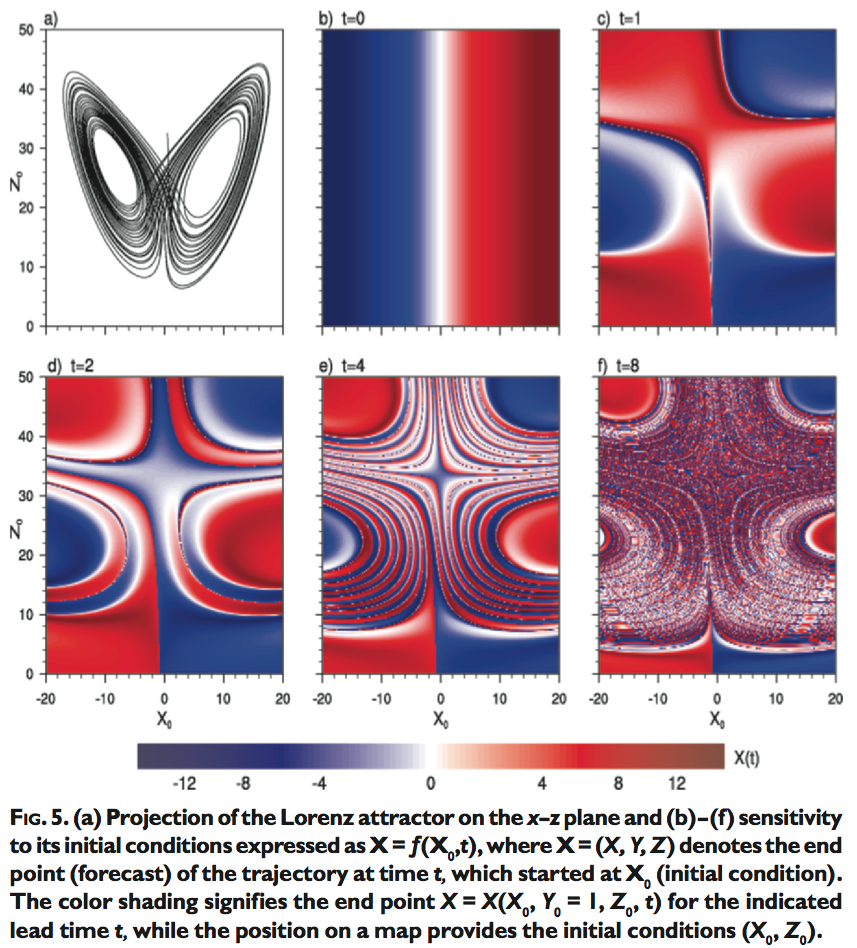
\includegraphics[height=33pc,width=33pc,angle=0]{figs/lorenz_attractor.png}
        \caption{\small Fig. 5 from \cite{hohenegger2007predictability}. (a) Projection of the Lorenz attractor on the $x$-$z$ plane and (b)–(f) sensitivity to its initial conditions expressed as $X = ƒ(X_0,t)$, where $X = (X, Y, Z)$ denotes the end point (forecast) of the trajectory at time $t$, which started at $X_0$ (initial condition). The color shading signifies the end point $X = X(X_0, Y_0 = 1, Z_0, t)$ for the indicated lead time t, while the position on a map provides the initial conditions $(X_0, Z_0)$.}
        \label{fig:lorenz}
    \end{center}
\end{figure}

